% !TeX spellcheck = en_US
\documentclass[sigconf,nonacm]{acmart}
\usepackage{listings}
\usepackage{tabularx}
\usepackage{siunitx}
\usepackage{subcaption}
\settopmatter{printacmref=false}
\pagestyle{empty}
\AtBeginDocument{%
  \providecommand\BibTeX{{%
    \normalfont B\kern-0.5em{\scshape i\kern-0.25em b}\kern-0.8em\TeX}}}
\copyrightyear{2020}
\acmYear{2020}
\setcopyright{rightsretained}
\begin{document}
\title{184.702 Security, Privacy and Explainability in Machine Learning}
\subtitle{Topic 3.3.1: Generation and Evaluation
of Synthetic Image Datasets}
\author{Thomas JIROUT}
\email{thomas.jirout@tuwien.ac.at}
\affiliation{Mat.Nr. 01525606}
\author{Helmuth BREITENFELLNER}
\email{helmuth.breitenfellner@student.tuwien.ac.at}
\affiliation{Mat.Nr. 08725866}
\begin{abstract}
In our third exercise for the lecture we are looking into
privacy-preserving data publishing.

As an example we are looking into a way of publishing image
data for training machine learning algorithms in the medical
domain, e.g.\ for
detecting diseases and anomalies.

Is it possible to replace a data set taken from real patients --
which can cause privacy-related issues -- with a set of images
generated from a GAN?
Can the generated data set be used for learning a network,
and what penalty in classification quality has to be
accepted for this approach?
These are the type of questions we want to answer in this exercise.
\end{abstract}
\maketitle

\section{Data Set}

We plan to take the data set from Kaggle\footnote{\url{https://www.kaggle.com/c/diabetic-retinopathy-detection}}
on
Diabetic Retinopathy Detection, published in 2015.

It contains images of the retina of eyes in varying resolution,
from $2600\times1900$ up to $5000\times3300$.

The training images are classified whether they are
depicting a Diabetic Retinopathy.
For this a scale from 0 to 4 is used.

For the test data there is no known ground truth -- it
was used for the original Kaggle
competition but has no value for this exercise.

The labeled data will be split into a holdout data set (20\%)
for evaluation
of the final learning and a training set (80\%).

\subsection{Preprocessing}

Most GANs need images of the same size, some of them requiring
the size to be a power of 2.
We therefore start with preprocessing each image
using \texttt{graphicsmagick}
to a square image of size $1024\times1024$.
\begin{lstlisting}[language=bash,basicstyle=\ttfamily\small]
gm convert -size 2048x2048 train/$FILE \
           -thumbnail 1024x1024^ -gravity center \
           -extent 1024x1024 +profile "*" \
           square/$FILE
\end{lstlisting}

Following this the images are to be preprocessed for the GAN
to be trained.
In the case of StyleGAN2 this would mean calling the
script \texttt{dataset\_tool.py} from their repository:
\begin{lstlisting}[language=bash,basicstyle=\ttfamily\small]
python dataset_tool.py create_from_images \
             ~/kaggle/tfdir ~/kaggle/square
\end{lstlisting}
\section{GAN}

A lot of GANs exist for the generation of images from a training set.
We decided to use
StyleGAN2\cite{stylegan2}
as it is a rather recent approach and the code is available on
GitHub\footnote{\url{https://github.com/NVlabs/stylegan2}}.

We were training five GANs, each for the classes (0-5).
For the image size we used $1024\times1024$ as the input and
also as the size of the generated images.
The training was performed by calling the script \texttt{run\_training.py}
(already part of StyleGAN2) from a wrapper script which uses a common
classification for all steps.

\subsection{Sample of Generated vs Real Images}

We were training the GANs for a parameter of \texttt{kimg=1000} -- which
is below the quality one would use for generating realistic images of persons,
but which we hoped would be already sufficient for training a classifier.

\begin{figure}[H]
\begin{subfigure}{0.18\linewidth}
\centering
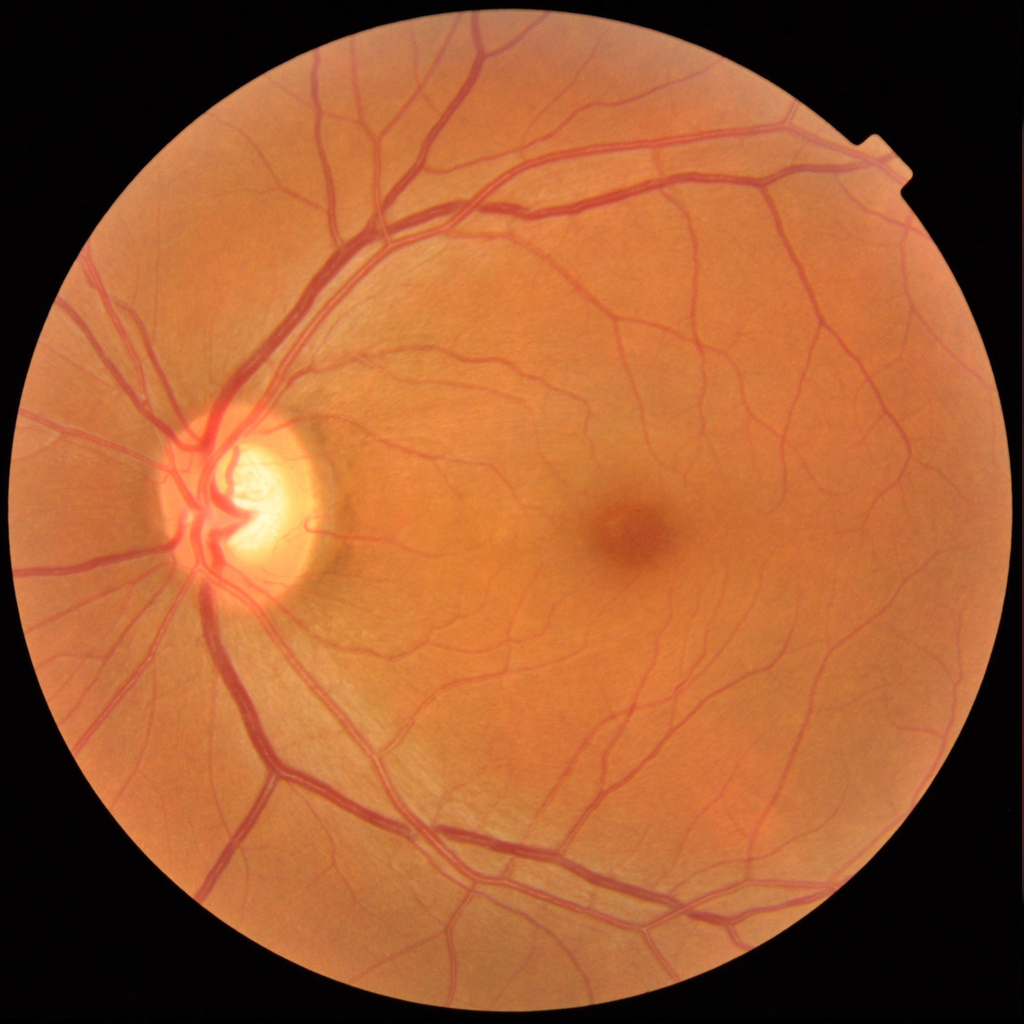
\includegraphics[width=0.9\linewidth]{real-class0.png}
\caption{Class 0}
\end{subfigure}
\begin{subfigure}{0.18\linewidth}
\centering
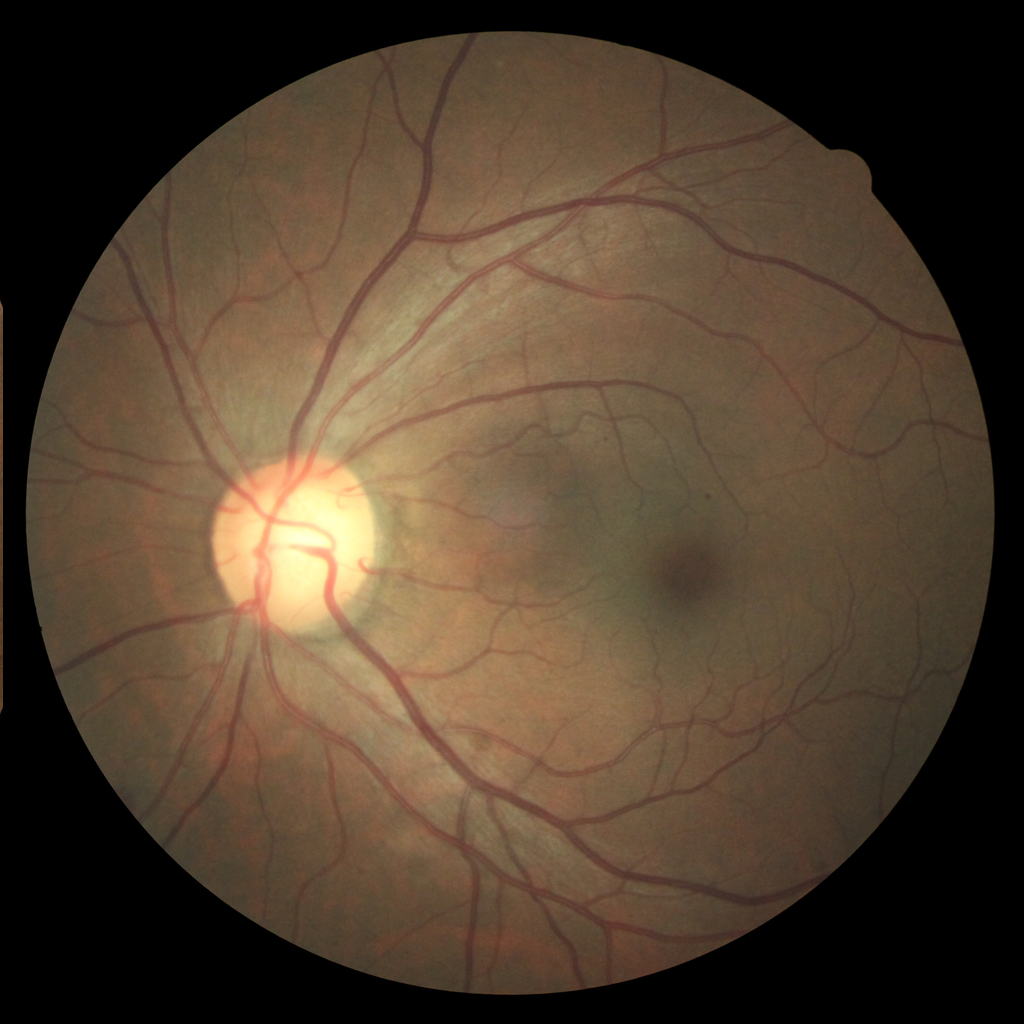
\includegraphics[width=0.9\linewidth]{real-class1.png}
\caption{Class 1}
\end{subfigure}
\begin{subfigure}{0.18\linewidth}
\centering
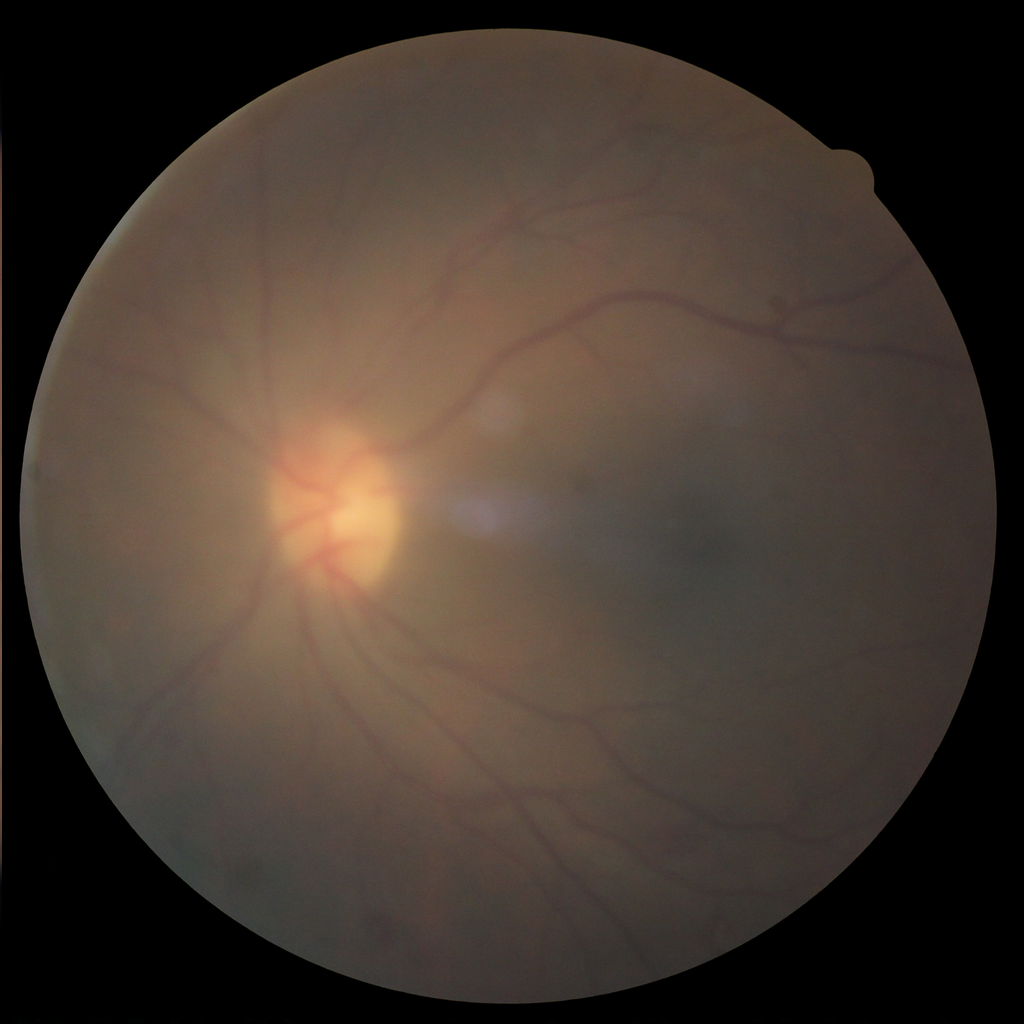
\includegraphics[width=0.9\linewidth]{real-class2.png}
\caption{Class 2}
\end{subfigure}
\begin{subfigure}{0.18\linewidth}
\centering
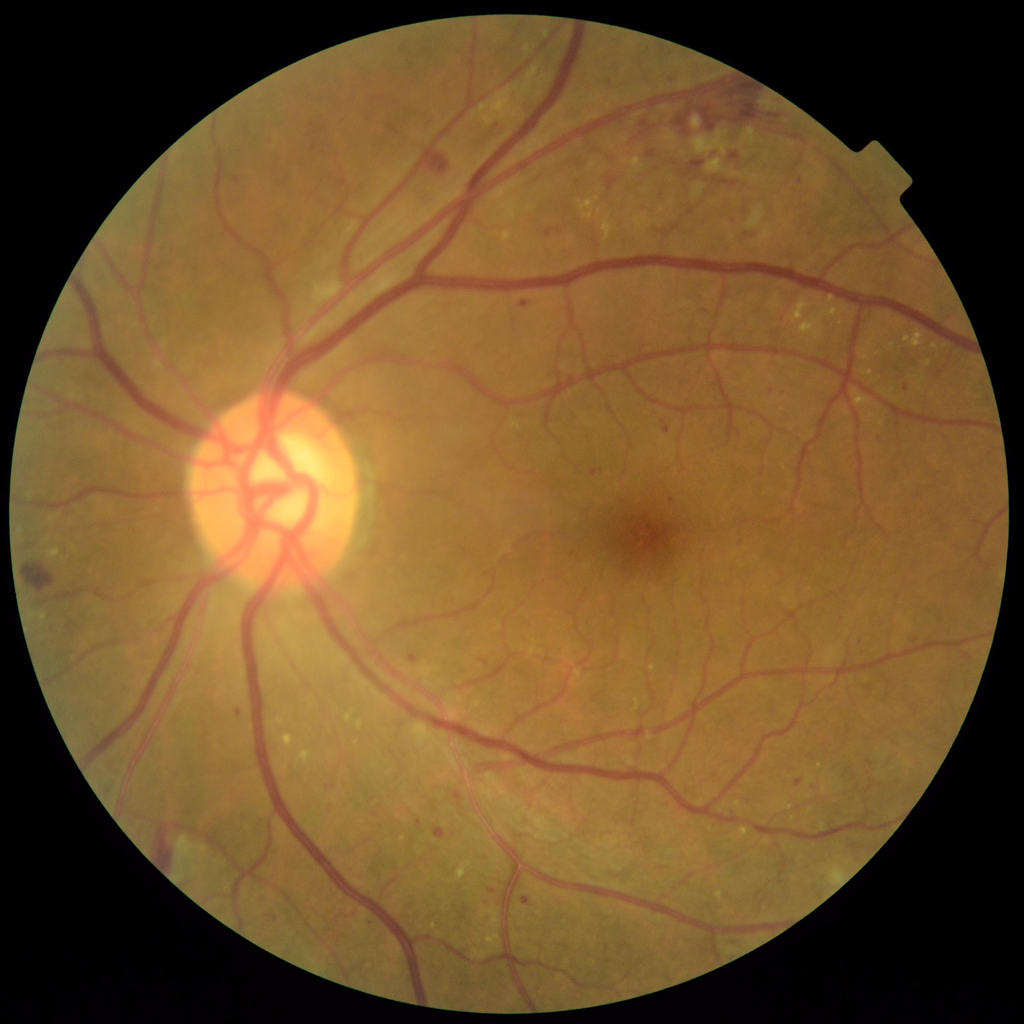
\includegraphics[width=0.9\linewidth]{real-class3.png}
\caption{Class 3}
\end{subfigure}
\begin{subfigure}{0.18\linewidth}
\centering
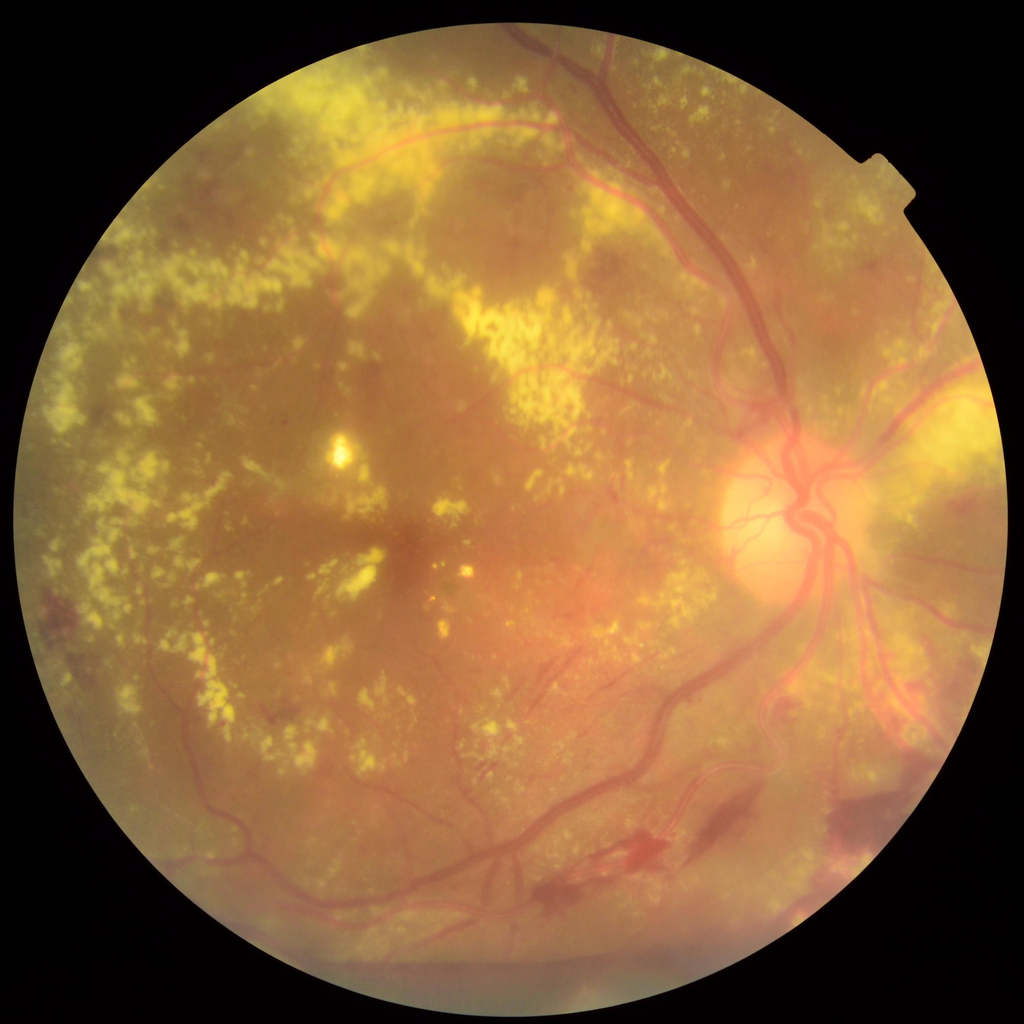
\includegraphics[width=0.9\linewidth]{real-class4.png}
\caption{Class 4}
\end{subfigure}
\caption{Samples of real images}
\label{fig:gan-real}
\end{figure}

\begin{figure}[H]
\centering
\begin{subfigure}{0.18\linewidth}
\centering
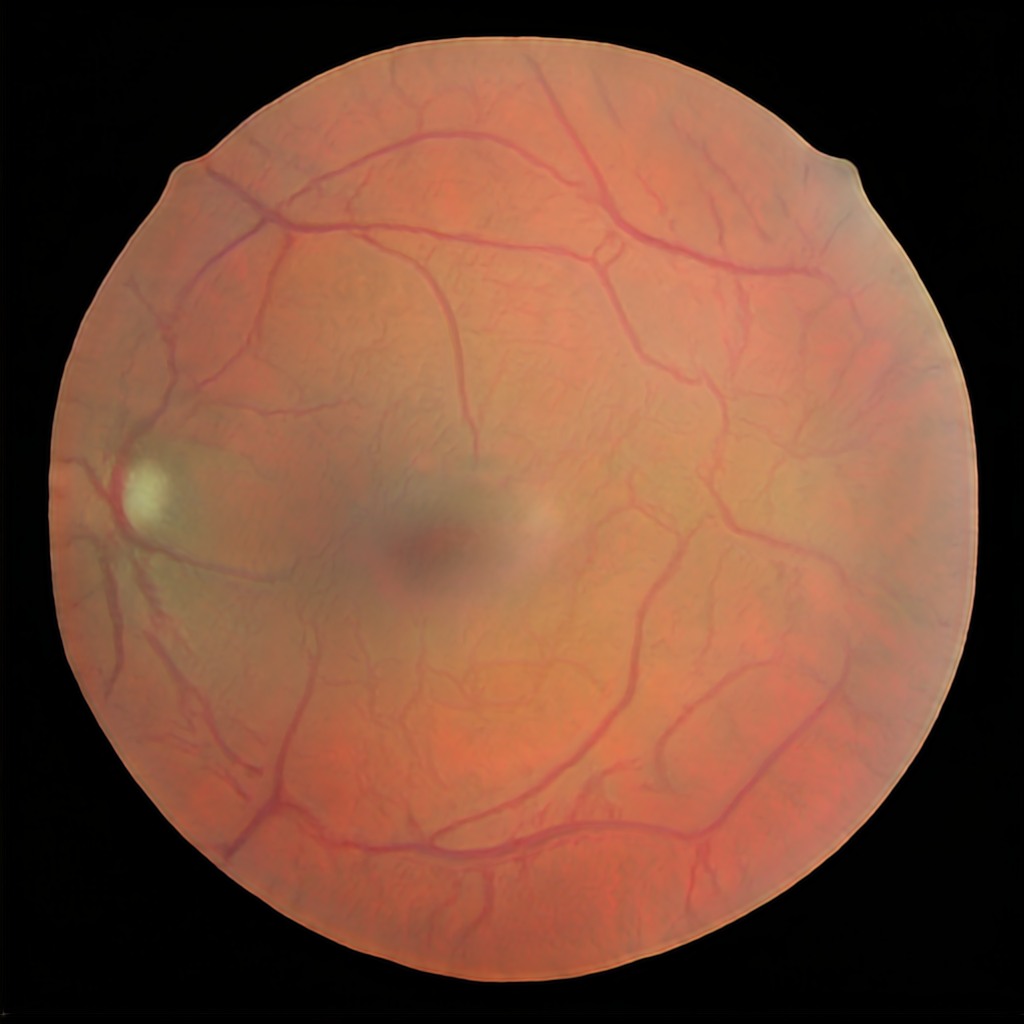
\includegraphics[width=0.9\linewidth]{fake-class0.png}
\caption{Class 0}
\end{subfigure}
\begin{subfigure}{0.18\linewidth}
\centering
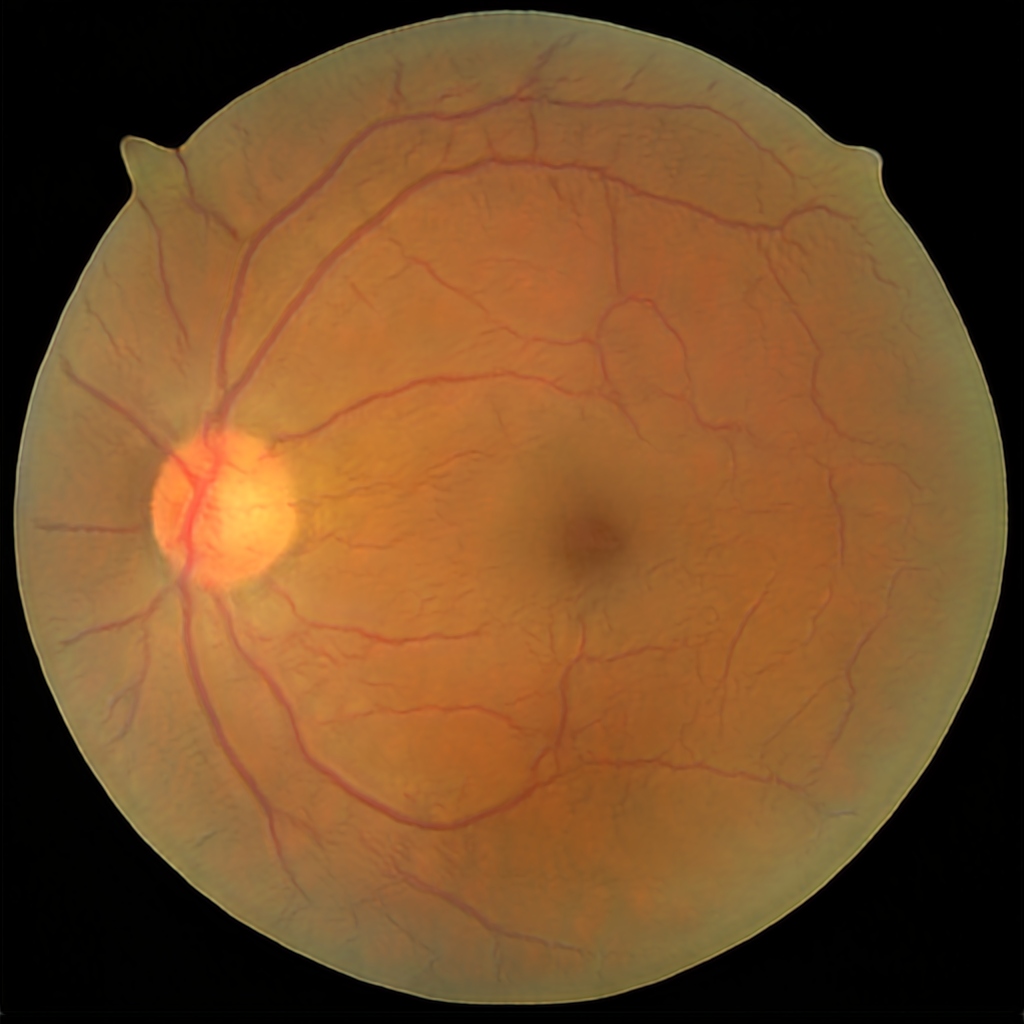
\includegraphics[width=0.9\linewidth]{fake-class1.png}
\caption{Class 1}
\end{subfigure}
\begin{subfigure}{0.18\linewidth}
\centering
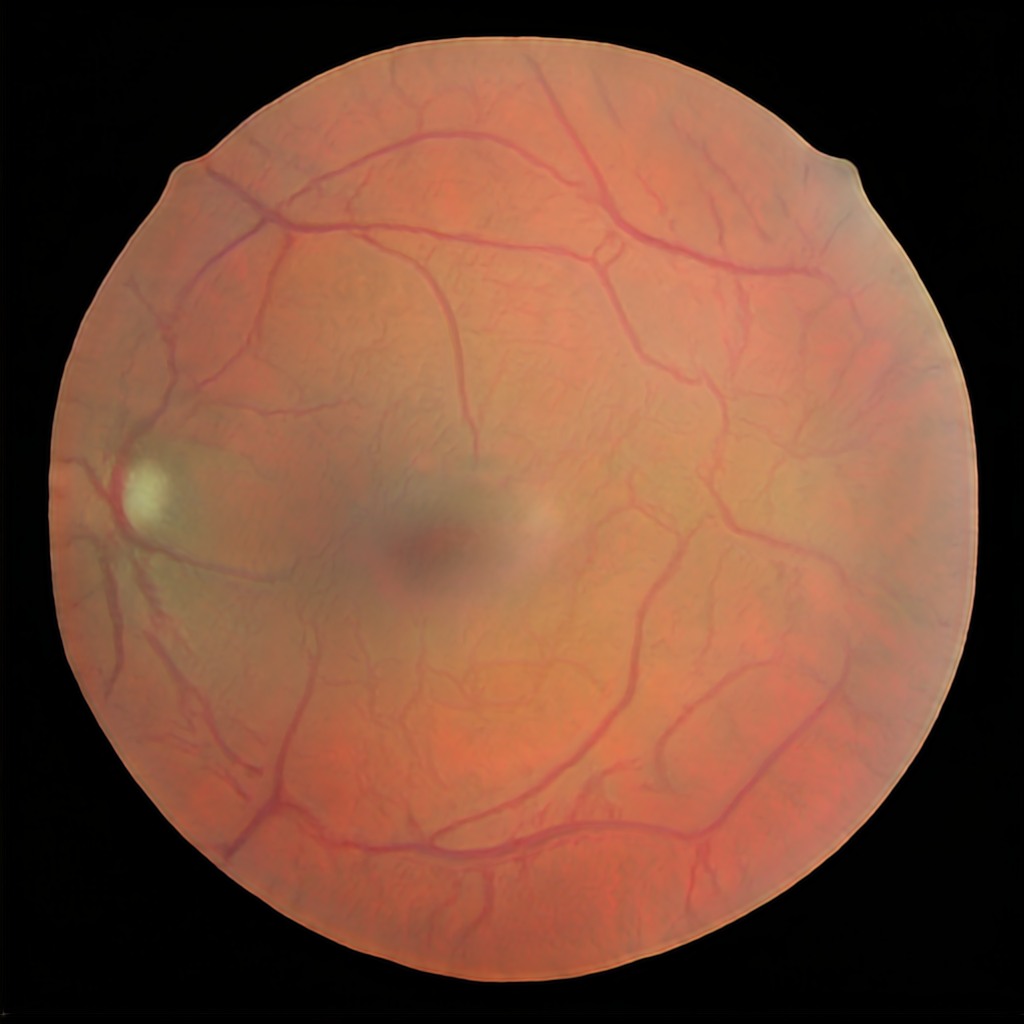
\includegraphics[width=0.9\linewidth]{fake-class0.png}
\caption{Class 2}
\end{subfigure}
\begin{subfigure}{0.18\linewidth}
\centering
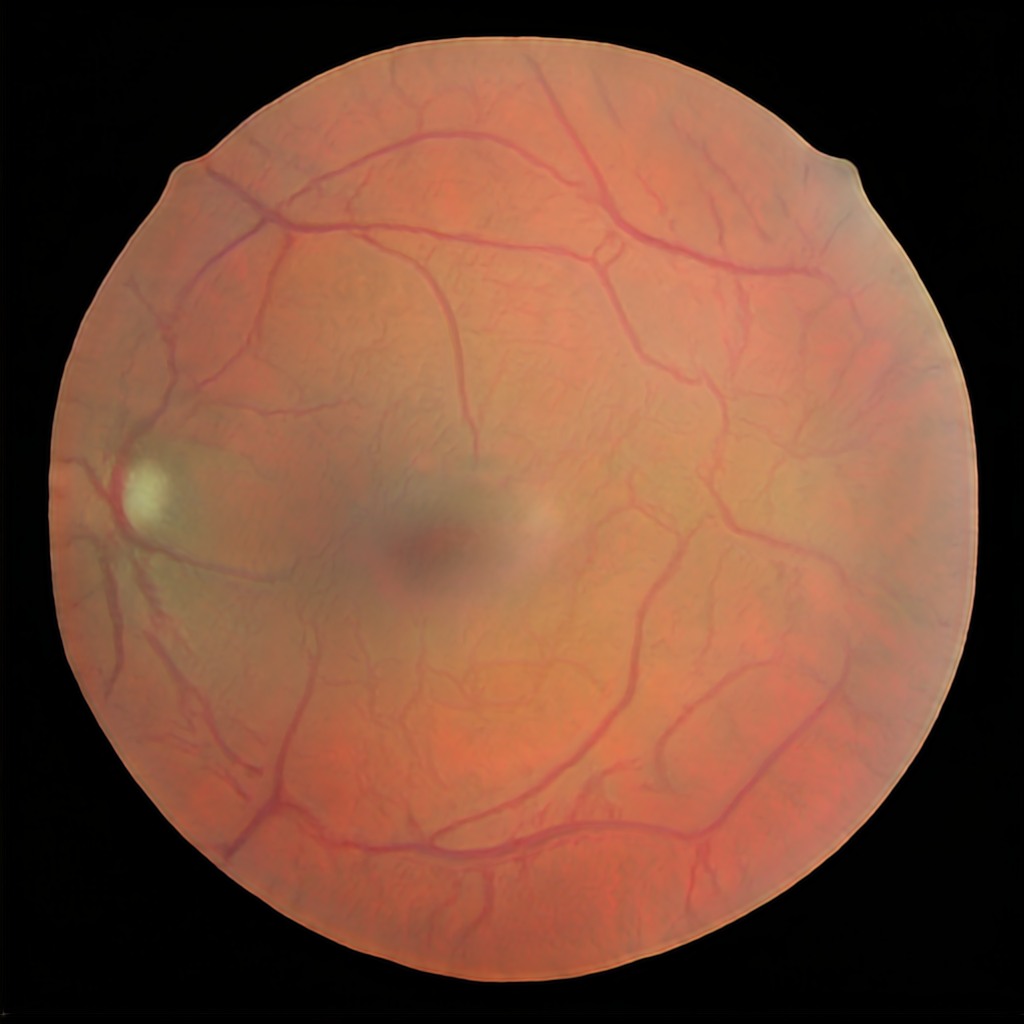
\includegraphics[width=0.9\linewidth]{fake-class0.png}
\caption{Class 3}
\end{subfigure}
\begin{subfigure}{0.18\linewidth}
\centering
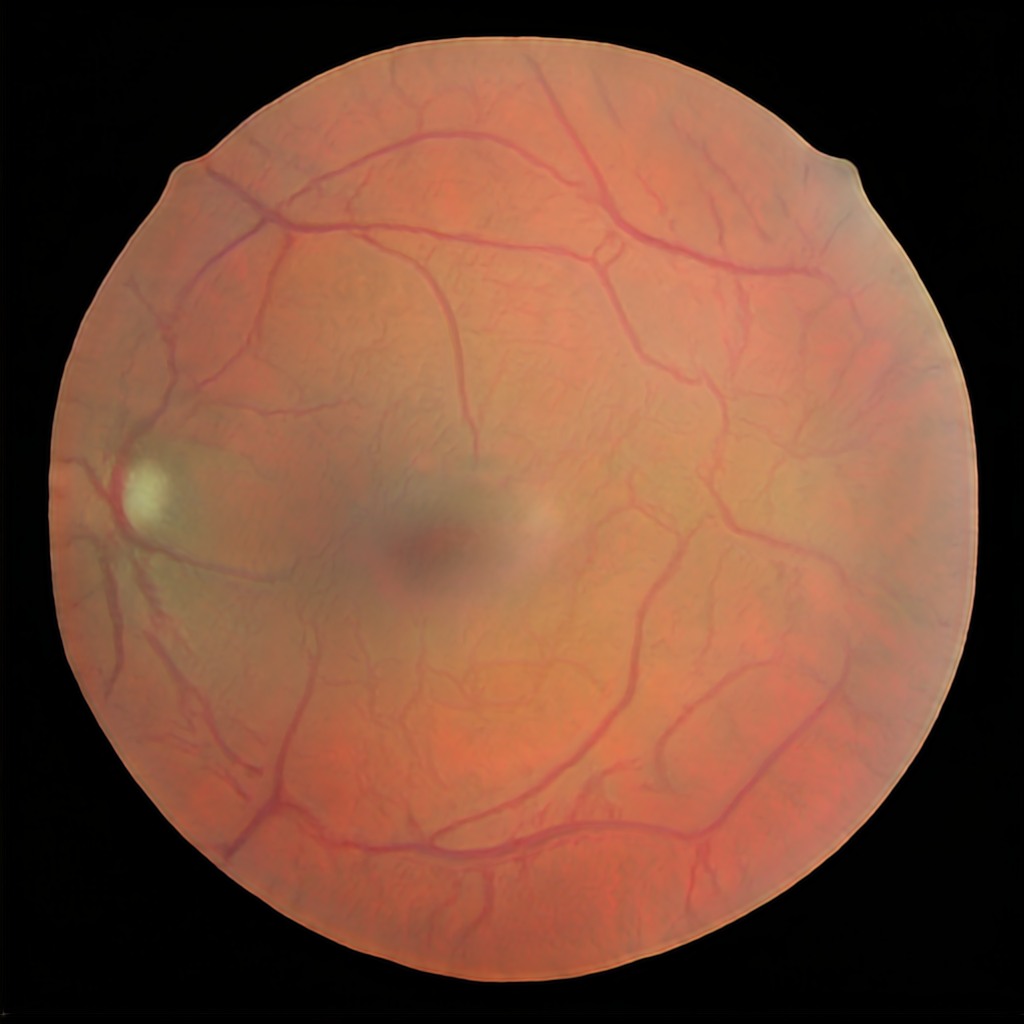
\includegraphics[width=0.9\linewidth]{fake-class0.png}
\caption{Class 4}
\end{subfigure}
\caption{Created (fake) images}
\label{fig:gan-fake}
\end{figure}

In summary a total of \SI{10000}{} samples were generated per class.

\section{Classifier}

For the classifier we were resorting to create our own classifier, based
on Convolutional Neural Network, using insight from the winning solution
\cite{kagglewinner}
of the Kaggle Competition.

\section{Evaluation}

The data set is highly imbalanced, therefore a simple
accuracy measure would not be appropriate.
Following the original
competition we plan to compare the quality of the classifiers
using the Quadratic Weighted
Kappa\footnote{\url{https://www.kaggle.com/aroraaman/quadratic-kappa-metric-explained-in-5-simple-steps}}.

This metric is a good choice for the problem, as the data set
is highly imbalanced, and also because the classes have an
inherent order.
Missing a class by one is of less concern than missing a class
by two or higher difference, and the quadratic
aspect in the metric takes care of penalizing higher differences
more.

\section{Risks \& Possible Problems}

There are a lot of risks, some technical, some knowledge-related.
We are listing some of the identified risks below.

At the end we will hopefully have learned a lot through this
experiment -- even if we fail with achieving a tangible result.

\subsection{Lack of Experience}

While this topic sounds super-interesting, we do not have
experience in the area of GANs and image processing in general
beyond basic CNNs for classification.

We do not plan to develop significant code for the exercise; still
our lack of experience will probably mean that we will need
more time for otherwise simple tasks, as we will have to
learn on-the-go.

\subsection{Computing Power \& Time}

We have access to a workstation with 4 NVIDIA Tesla V100 for
the exercise.
Still the training time might be beyond what we can afford.
From the original paper and based on the capacity available
to us, we expect a training time of about 1 week if we use
a subset of \SI{10000}{} images.
This is for learning the GAN -- we hope that learning the
classifier will need significantly less time.

If necessary, we plan to make some further simplifications for
countering these issues.
We might use 256x256 images instead, or use less from the data set,
to come up with results within the provided time limit.

We plan to document and provide code for the experiment in a way
which allows later a more complete run, with the full data set
and highest possible resolution.

\subsection{Insufficient Data}

There are \SI{35126}{} images in the data set.
This might turn out to be not
sufficient, especially for some of the classes (e.g.\ in class 4
there are only 709 samples).
This might force us to do some simplification, like using only two
classes by combining them together.

We might also use data augmentation. StyleGAN2 has support for
augmentation by mirroring the images which can be activated
via a flag.

Another possibility is using a staged approach: first learning
one network on the whole data set of all images, then
cloning it for the classes and ``fine-tuning'' it on the subset
of images.

\subsection{Implementation Issues}

Especially for older code it is often quite difficult to
make it run using modern library versions.
Methods might have been deprecated in the meantime and cannot
be used anymore.

We will try to work around this type of issues, and in many cases
we should be able to use different approaches (e.g.\ different
classifiers) for the purpose of the exercise.

For the preparation of this concept we started running some
of the steps, like training the GAN.
We hope that this way we encounter implementation issues early on
so we can resolve them in time.

\bibliographystyle{ACM-Reference-Format}
\bibliography{report}
\end{document}
